% !TEX root = Heuberger_Petracci_reflID_735.tex

\begin{figure}[ht]
\centering
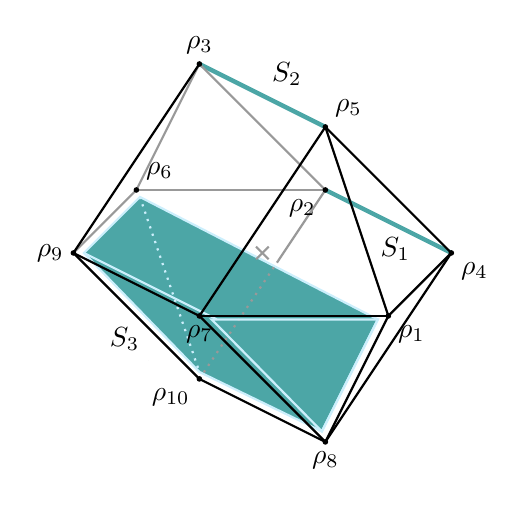
\begin{tikzpicture}[scale=0.8,every node/.style={scale=1}]

\filldraw[color=cyan!20, fill=blue!50!green!70, thick] (-2+1/18,1-2/18) -- (2-3/18,-1-1/18) -- (1-1/18,-3+3/18) -- (-1,-2+2/18) -- (-3+3/18,0) -- cycle; 
\draw[ultra thick, blue!50!green!70] (1,1) -- (3,0);
\draw[ultra thick, blue!50!green!70] (-1,3) -- (1,2);
\draw[thick, dotted, cyan!20] (-2+1/18,1-2/18) --  (-1,-2+2/18);

%background edges
\draw[gray!80, thick] (1,1) -- (-2,1);
\draw[gray!80, thick] (1,1) -- (-1,3);
%\draw[gray!80, thick] (1,1) -- (3,0);
\draw[gray!80, thick] (-1,3) -- (-2,1);
\draw[gray!80, thick] (-3,0) -- (-2,1);
\draw[gray!80, thick] (1,1) -- (1/4,-1/8);
\draw[gray!80, dotted, thick] (1/4,-1/8) -- (-1,-2);
%\draw[gray!80, dashed, thick] (-1,-2) -- (-2,1);

\draw[thick, cyan!20] (2-3/18,-1-1/18) -- (-1+3.5/18,-1-1/18) --   (1-1/18,-3+3/18)  -- cycle;
\draw[thick, cyan!20]  (-3+3/18,0)  -- (-1+5/18,-1-1/18);

%foreground edges
\draw[black, thick] (-3,0) -- (-1,3);
\draw[black, thick] (-3,0) -- (-1,-1);
\draw[black, thick] (-1,-1) -- (1,2);
\draw[black, thick] (1,2) -- (3,0);
\draw[black, thick] (1,2) -- (2,-1);
\draw[black, thick] (-1,-1) -- (2,-1);
\draw[black, thick] (2,-1) -- (3,0);
%\draw[black, thick] (1,2) -- (-1,3);
\draw[black, thick] (3,0) -- (1,-3);
\draw[black, thick] (2,-1) -- (1,-3);
\draw[black, thick] (-1,-2) -- (1,-3);
\draw[black, thick] (-1,-2) -- (-3,0);
\draw[black, thick] (-1,-1) -- (1,-3);

%origin 
\draw[gray!80, thick] (0.1,0.1) -- (-0.1,-0.1);
\draw[gray!80, thick] (-0.1,0.1) -- (0.1,-0.1);


%nodes
\filldraw[black] (2,-1) circle (1pt) node[anchor=north west] {$\rho_1$};
\filldraw[black] (3,0) circle (1pt) node[anchor=north west] {$\rho_4$};
\filldraw[black] (1,1) circle (1pt) node[anchor=north east] {$\rho_2$};
\filldraw[black] (-2,1) circle (1pt) node[anchor=south west] {$\rho_6$};
\filldraw[black] (-3,0) circle (1pt) node[anchor=east] {$\rho_9$};
\filldraw[black] (1,-3) circle (1pt) node[anchor=north] {$\rho_8$};
\filldraw[black] (-1,-2) circle (1pt) node[anchor=north east] {$\rho_{10}$};
\filldraw[black] (1,2) circle (1pt) node[anchor=south west] {$\rho_5$};
\filldraw[black] (-1,3) circle (1pt) node[anchor=south] {$\rho_3$};
\filldraw[black] (-1,-1) circle (1pt) node[anchor=north ] {$\rho_7$};


\filldraw[black] (2.5,0.4) circle (0pt) node[anchor=north east] {$S_1$};
\filldraw[black] (0,2.5) circle (0pt) node[anchor=south west] {$S_2$};
\filldraw[black] (-1.8,-1.7) circle (0pt) node[anchor=south east] {$S_3$};


%\filldraw[black] (5,-3) circle (1pt) node[anchor=north west] {$(1,1,-1)$};
%\filldraw[gray] (2,-2) circle (1pt) node[label={[xshift=-0.9cm, yshift=-0.3cm]\textcolor{black}{$(0,1,-1)$}}]{};
%\filldraw[gray] (-6,-7) circle (1pt) node[label={[xshift=1.3cm, yshift=-0.3cm]\textcolor{black}{$(-1,-2,-2)$}}]{};
%\filldraw[black] (-2,-10) circle (1pt) node[anchor=north] {$(1,-3,-2)$};
%
%\filldraw[gray] (0,-3) circle (1pt) node[anchor=south east]{};
\end{tikzpicture}

\caption{Scaffolding of P735}
\label{ScaffoldingP735}

\end{figure}

